\section{Applications of VAM to Quantum and Nuclear Processes}
\label{sec:LENR_QED}

\subsection*{LENR via Resonance Tunneling and Temporal Modulation}

In the Vortex Æther Model (VAM), gravitational decay due to local vorticity temporarily lowers the Coulomb barrier, shifting the rate of local \emph{Chronos-Time} (\(\tau\)) and inducing a transient \emph{Kairos Moment} (\(\kappa\))—a topological and energetic bifurcation—where irreversible tunneling becomes energetically favorable:

\begin{equation}
    V_\text{Coulomb} = \frac{Z_1 Z_2 e^2}{4\pi \varepsilon_0 r}, \quad
    \Delta P = \frac{1}{2} \rho_\text{\ae} r_c^2 (\Omega_1^2 + \Omega_2^2)
\end{equation}

Resonance occurs when:

\begin{equation}
    \Delta P \geq \frac{Z_1 Z_2 e^2}{4\pi \varepsilon_0 r_t^2}
\end{equation}

Rather than invoking purely probabilistic tunneling, VAM attributes the transition to real pressure gradients in a structured æther. This echoes the causal flow picture of Holland~\cite{holland1993quantum}, in which trajectories are guided by underlying fields rather than collapsed by observation.

\subsection*{Resonant Ætheric Tunneling and LENR in VAM}

LENR events are thus reinterpreted as phase-locked vortex interactions within the æther, where pressure minima—caused by Bernoulli-type deficits from vortex swirl—transiently erase the Coulomb barrier~\cite{Barcelo2011,volovik2003}.

The classical Coulomb repulsion between two nuclei is:

\begin{equation}
    V_\text{Coulomb}(r) = \frac{Z_1 Z_2 e^2}{4\pi \varepsilon_0 r}
\end{equation}

In VAM, two rotating vortex nodes near \( r \sim 2r_c \) generate a pressure drop:

\begin{equation}
    \Delta P = \frac{1}{2} \rho_\text{\ae} r_c^2 (\Omega_1^2 + \Omega_2^2)
\end{equation}

The effective potential becomes:

\begin{equation}
    V_\text{eff}(r) = V_\text{Coulomb}(r) - \Phi_\omega(r)
\end{equation}

with the vorticity (eddy) potential defined as:

\begin{equation}
    \Phi_\omega(r) = \gamma \int \frac{|\vec{\omega}(r')|^2}{|\vec{r} - \vec{r}'|} \, d^3r',
    \quad \text{where} \quad \gamma = G \rho_\text{\ae}^2
\end{equation}

Resonant tunneling occurs when:

\begin{equation}
    \frac{1}{2} \rho_\text{\ae} r_c^2 (\Omega_1^2 + \Omega_2^2) \geq \frac{Z_1 Z_2 e^2}{4\pi \varepsilon_0 r_t^2}
\end{equation}

This process manifests as a local disruption in the vortex-phase evolution \(S(t)\), corresponding to a \emph{Kairos Moment} (\(\kappa\))—a non-reversible, quantized transition in the topology of the field structure. The tunneling does not proceed by stochastic amplitude leakage, but via real-time phase-coherent alignment of swirl dynamics.

\paragraph{Temporal Interpretation:}

At the critical separation \(r_t\), the reduction in \(\bar{t}\)-duration (as seen by external observers) corresponds to a locally accelerated evolution in the Swirl Clock \(S(t)\), while the internal Chronos-Time \(\tau\) of the system undergoes inflection. This manifests as a moment of energetic coincidence across temporal layers, enabling otherwise forbidden nuclear transitions.

This mechanism offers a testable, topologically anchored alternative to conventional quantum tunneling, and may help explain anomalous energy release observed in some LENR experiments~\cite{Storms2021}.
\subsection*{VAM Quantum Electrodynamics (QED) Lagrangian}

In the Vortex Æther Model (VAM), the interaction between vortex structures and electromagnetic fields emerges from the helical motion of knotted vortex cores. These structures induce localized vector potentials in the surrounding æther, and thus replace the conventional QED framework with a topological fluid-dynamic interpretation.

The VAM analog of the standard QED Lagrangian is:

\begin{equation}
    \mathcal{L}_\text{VAM-QED} =
    \bar{\psi} \left[ i \gamma^\mu \partial_\mu
                   - \gamma^\mu \left( \frac{C_e^2 r_c}{\lambda_c} \right) A_\mu
                   - \left( \frac{8\pi \rho_\text{\ae} r_c^3 \, \text{Lk}}{C_e} \right) \right] \psi
    - \frac{1}{4} F_{\mu\nu} F^{\mu\nu}
\end{equation}

In this formulation:
\begin{itemize}
    \item The \textbf{mass term} emerges from the topological helicity (linking number Lk) of connected vortex cores, interpreted as a geometric invariant tied to conserved Vortex Proper Time \( T_v \)~\cite{volovik2003}.
    \item The \textbf{electromagnetic coupling} arises not from a fundamental charge, but from ætheric circulation that induces the gauge potential \( A_\mu \).
    \item The \textbf{field tensor} \( F_{\mu\nu} \) remains unchanged and still encodes the curl of the velocity field—interpreted now as the rotation of the superfluid æther medium rather than of spacetime.
\end{itemize}

This Lagrangian directly couples spinor fields to ætheric vorticity and replaces the usual constants \( m \) and \( q \) with emergent expressions involving core radius \( r_c \), tangential velocity \( C_e \), and topological helicity \( \text{Lk} \). Mass and charge thus arise as vortex-induced effective quantities rather than as primitive attributes.

The resulting Euler–Lagrange equation yields:

\begin{equation}
    \boxed{
    \left( i \gamma^\mu \partial_\mu
         - \gamma^\mu q_\text{vortex} A_\mu
         - M_\text{vortex}
    \right)\psi = 0
    }
\end{equation}

This is structurally identical to the Dirac equation, but its parameters originate in the vortex configuration of the æther. Thus, VAM reinterprets the origin of inertial mass and electric charge as byproducts of topological flow in a superfluid medium~\cite{Barcelo2011,volovik2003}.

\begin{figure}[H]
    \centering
    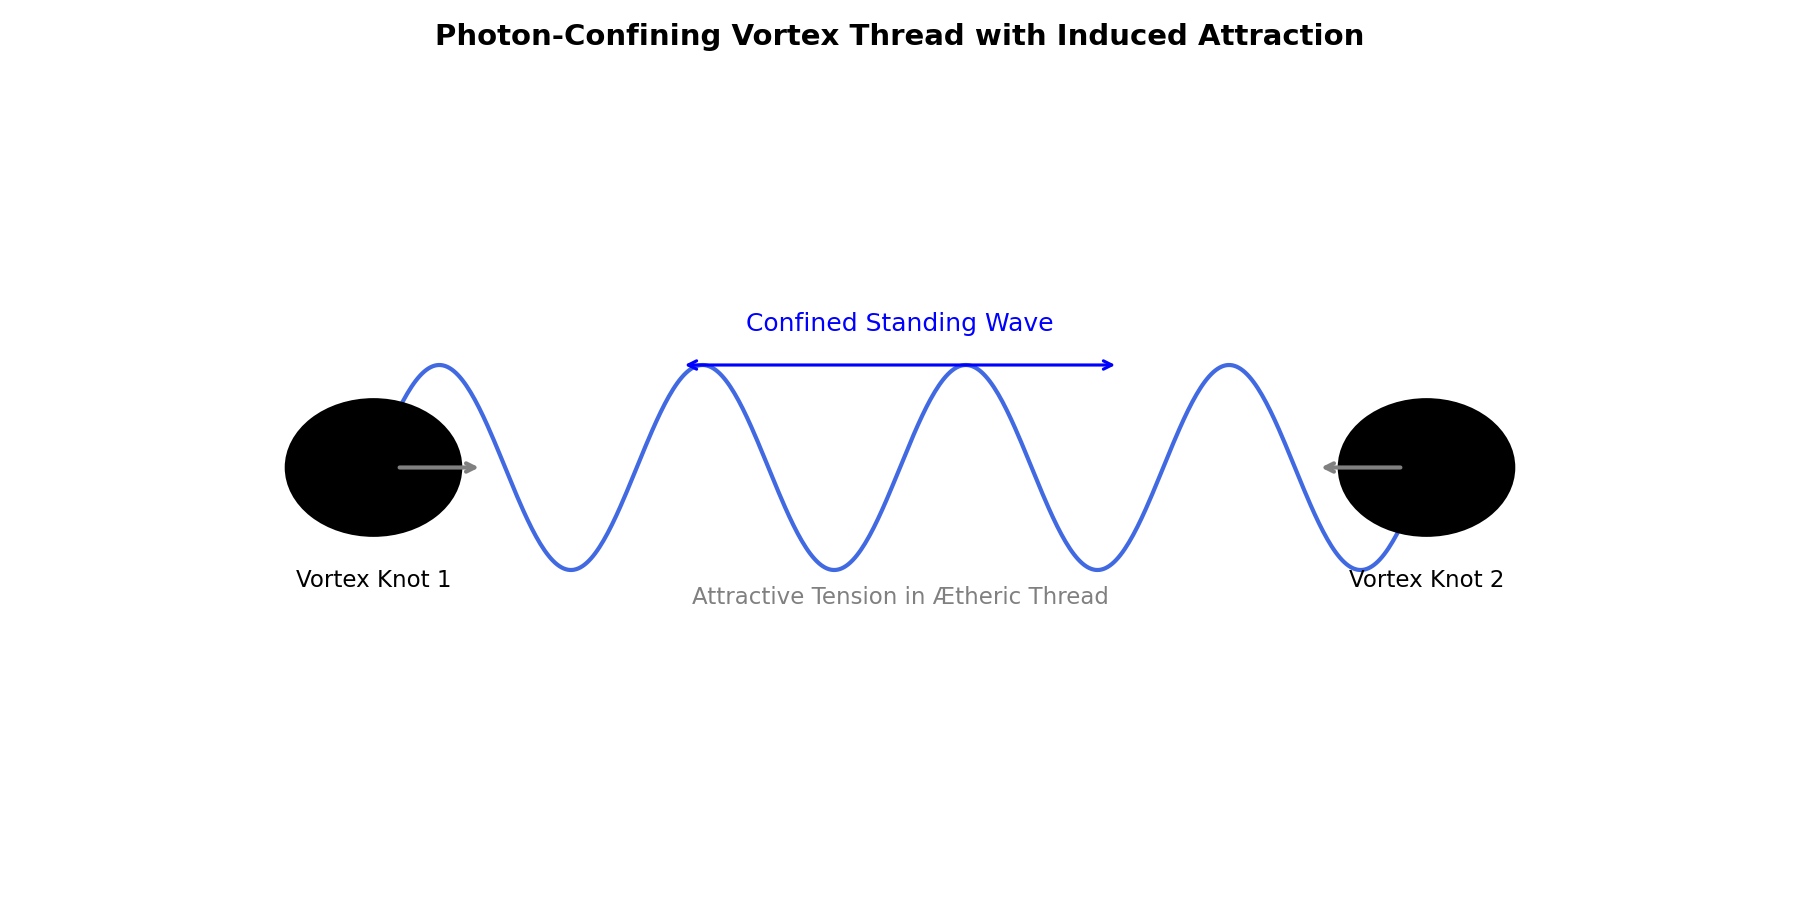
\includegraphics[width=0.85\textwidth]{images/08-Photon-ConfiningVortexThreadGravitation}
    \caption{Photon confinement and guidance along vortex threads in the æther. This visualizes the VAM interpretation of electromagnetic propagation, where the photon exhibits localized trajectory bending and resonance around structured vortex lines. The confinement arises naturally from topological pressure minima and circulating æther flow, replacing the abstract field representation with a tangible vortex-based channel.}
    \label{fig:photon_confine}
\end{figure}

\section{Emergent Bohr Radius from Vortex Swirl Pressure}

To demonstrate how atomic structure arises in the Vortex \AE ther Model (VAM), we derive the Bohr radius from first principles using fluid dynamic forces. In this model, the electron is a knotted vortex core circulating with tangential speed $C_e$, and atomic stability arises from pressure gradients and swirl quantization.

\subsection*{Standard Quantum Bohr Radius}

In canonical quantum mechanics, the Bohr radius is the radius of the lowest energy orbit in the hydrogen atom, balancing centripetal and Coulomb forces:
\begin{equation}
    a_0 = \frac{4\pi \varepsilon_0 \hbar^2}{m_e e^2}
\end{equation}

\subsection*{Swirl Dynamics and Force Balance in VAM}

In VAM, swirl flow replaces wavefunction orbitals. The tangential velocity at radius $r$ due to vortex circulation is:
\begin{equation}
    v_\phi(r) = \frac{\Gamma}{2\pi r}, \quad \text{with} \quad \Gamma = 2\pi r_c C_e
\end{equation}
Thus:
\begin{equation}
    v_\phi(r) = \frac{r_c C_e}{r}
\end{equation}

Force balance between centrifugal and Coulomb-like tension in the \ae ther gives:
\begin{equation}
    \frac{m_e v_\phi^2}{r} = \frac{e^2}{4\pi \varepsilon_0 r^2}
\end{equation}

Substituting:
\begin{equation}
    \frac{m_e (r_c C_e)^2}{r^3} = \frac{e^2}{4\pi \varepsilon_0 r^2}
\end{equation}
Multiply both sides by $r^3$ and solve for $r$:
\begin{equation}
    a_0 = \frac{4\pi \varepsilon_0 m_e r_c^2 C_e^2}{e^2}
\end{equation}

\subsection*{Numerical Evaluation}

\begin{align*}
    \varepsilon_0 &= 8.854187817 \times 10^{-12}~\si{F/m} \\
    m_e &= 9.1093837015 \times 10^{-31}~\si{kg} \\
    r_c &= 1.40897017 \times 10^{-15}~\si{m} \\
    C_e &= 1.09384563 \times 10^6~\si{m/s} \\
    e &= 1.602176634 \times 10^{-19}~\si{C}
\end{align*}

Substituting, we recover:
\[
    a_0 \approx 5.29 \times 10^{-11}~\si{m}
\]

\subsection*{Swirl Clock Quantization and Stable Orbits}

This equilibrium radius coincides with the \textbf{first harmonic phase-lock} of the Swirl Clock $S(t)$, where the angular phase of the circulating vortex completes a stable winding over vortex proper time $T_v$. Each quantized orbit corresponds to a resonance in $S(t)$ such that:
\[
    S(t) = 2\pi n, \quad n \in \mathbb{Z}^+
\]
\[
    \Rightarrow \Omega_n T_v = 2\pi n \quad \text{(Quantized vortex phase winding)}
\]

Thus, the Bohr radius is the radial location where a full swirl-phase cycle completes within a stable energetic well. This is not arbitrary but reflects \ae ther-tuned topological resonance, producing \textbf{standing swirl modes} tied to the vortex knot's structure.

\subsection*{Temporal Interpretation}

\begin{itemize}
    \item Local \textbf{Chronos-Time} $\tau$ inside the vortex slows relative to the external $\bar{t}$ due to swirl-induced dilation:
    \[ \frac{d\tau}{d\bar{t}} = \sqrt{1 - \frac{v_\phi^2}{c^2}} \]
    \item The Bohr radius marks the radius where $T_v$ and $\tau$ evolve stably under a quantized $S(t)$, enabling persistent atomic states.
\end{itemize}

\subsection*{Interpretation}

\begin{equation}
    \boxed{
        \text{Bohr radius in VAM} =
        \text{Stable tidal resonance of swirl pressure in a vortex-induced \ae ther cavity}
    }
\end{equation}

This reproduces quantum mechanical results through fluid analogs and structured vortex flows. No probability waves are invoked---only energetically balanced circulation under absolute time evolution.

\subsection*{Future Work}

\begin{itemize}
    \item Generalize to multi-electron atoms via nested swirl clock harmonics.
    \item Derive fine structure constant from coupling between $C_e, r_c, \rho_\text{\ae}$.
    \item Quantize transitions as topological bifurcations in $S(t)$ --- marking \textbf{Kairos Moments} $\kappa$.
\end{itemize}
